In order to create smaller patches which still contain the described relationships, we turn to the foraging concept of scent. Following the example of WUFIS and PFIS, we define the foraging concept \textit{Information Scent} as the ``inferred relatedness of a cue to the prey, as measured by amount of activation from a spreading activation algorithm.'' In WUFIS and PFIS, relatedness between two nodes was determined by a function of textual similarity and encoded into the weights of the edge connecting those two nodes. The application of spreading activation introduced a notion of proximity; each node's activation is representative of its textual similarity and proximity to the starting point\textemdash the information need. Our challenge is taking the work of WUFIS and PFIS and defining these concepts in our socio-technical context. Once we have a measure of relatedness in traceability foraging, we can create patches.

\section{Spreading Activation over Requirements Socio-Technical Graphs}
If a forager posts a question on an issue, the user who will provide the answer will likely require knowledge on that issue. From this postulate, we define our notion of ``relatedness'' between two nodes: the degree of a user's relatedness to an artifact is proportional to their knowledge on the artifact. This serves as an analogue to PFIS's textual similarity. The user's knowledge on an artifact is encoded as the weight on the edge connecting them. Note that, to support our implementation of spreading activation, a lower weight represents a more powerful connection.
\begin{itemize}
  \item \textit{Comment to Issue, Question to Issue:} \textbf{weight = 1}. This is the only type of artifact-to-artifact edge we defined in our RSTGs. If a comment or question is posted to an issue, it is directly a part of the traceability history of that issue. Therefore, its connection to the issue should be extremely strong.
  \item \textit{Creator to Issue, Assignee to Issue:} \textbf{weight = 2}. As discussed, the creator and assignee have a high degree of knowledge on a given issue. In relationships connecting question to answer, the assignee or creator frequently answered questions if the forager did not directly reference a user first (Figure \ref{fig:pie}: 55\% of questions). However, an issue can develop without the supervision of the creator or assignee. Therefore, the connection of this relationship is lower than that of an issue to a comment.
  \item \textit{Comment to Referenced:}  \textbf{weight = 2}. The user who wrote the comment has determined that the referenced user should have strong knowledge on the comment. Figure \ref{fig:pie} shows that 31\% of questions were answered by a referenced user; this relationship is therefore prioritized with a strong connection.
  \item \textit{Comment to User:} \textbf{weight = 3}. While the connection of a comment to the issue is strong, the user is not guaranteed to have knowledge on the issue to the same degree as Creator or Assignee. Therefore, we set the user's connection to the issue lower than that of a creator or assignee.
  \item \textit{Question to User:} \textbf{weight = 4}. Questions, like comments, do not guarantee knowledge on the issue. If anything, a user asking a question is least-qualified of the users discussed to provide an answer. Therefore, we give this relationship the weakest connection.
\end{itemize}

With weight defining the relatedness between two given nodes, now a given node's relatedness to the forager's information need can be determined. The classes discussed in the previous section demonstrated that answers fell within four degrees of separation, and that answers were likely to come from Frequent Collaborators. These concepts can be encoded by adapting spreading activation.


\begin{algorithm}
	\textbf{Spreading Activation}
	\begin{algorithmic}[1]
		\renewcommand{\algorithmicrequire}{\textbf{Input:}}
 		\renewcommand{\algorithmicensure}{\textbf{Output:}}
		\REQUIRE Graph, Source Node 
		\ENSURE Graph with Activated Nodes
		\STATE $Decay \leftarrow 0.1$
		\STATE $source.activation\leftarrow 1$
			\FOR{$node$ in Breadth-First Traversal from $source$}
				\FOR{$preNode$ in Neighbors of $node$}
					\IF{$preNode$ has been traversed}
						\STATE $weight \leftarrow edge(preNode,node)$
						\STATE $newActivation \leftarrow preNode.activation * (1 - weight * decay)$
						\STATE $node \leftarrow Activate(node, newActivation)$
					\ENDIF
				\ENDFOR
			\ENDFOR
	\end{algorithmic}
	~\\
	\textbf{Co-Routine: Activate}
	\begin{algorithmic}[1]
		\renewcommand{\algorithmicrequire}{\textbf{Input:}}
 		\renewcommand{\algorithmicensure}{\textbf{Output:}}
		\REQUIRE Node, New Activation
		\ENSURE Activated Node
		\STATE $frequencyReward \leftarrow 0.01$
		\IF{$node$ has activation}
			\STATE $maxAct \leftarrow max(node.activation, newAct)$
			\STATE $minAct \leftarrow min(node.activation, newAct)$
			\STATE $node.activation \leftarrow maxAct + ((1-maxAct) * minAct * frequencyReward)$
		\ELSE
			\STATE $node.activation \leftarrow newActivation$
		\ENDIF
	\end{algorithmic}
\caption{Spreading Activation over an RSTG}
\label{alg:spread}'
\end{algorithm}

As shown in Algorithm \ref{alg:spread}, our variant of spreading activation starts at the question-node. The question's activation is set to 1. Then, surrounding nodes are traversed (Algorithm \ref{alg:spread}, Line 3), and activation is spread from their predecessors (Algorithm \ref{alg:spread}, Lines 4-8). Spreading activation traditionally has each node firing to its successors; our predecessor variant exhibits greater decay while still producing useful networks. Our exact mechanism of spreading activation is shown in Algorithm \ref{alg:spread}, Line 7, and the Algorithm \ref{alg:spread} Co-Routine.

Line 7 shows how exactly weight is factored in. A lower weight implies a higher degree of relatedness. If activation is a measure of relatedness, lower weights should result in higher activations. Therefore, the lower the weight, the smaller the effect of the decay, and the higher the resulting activation.

\begin{figure}[ht]
	\centering
	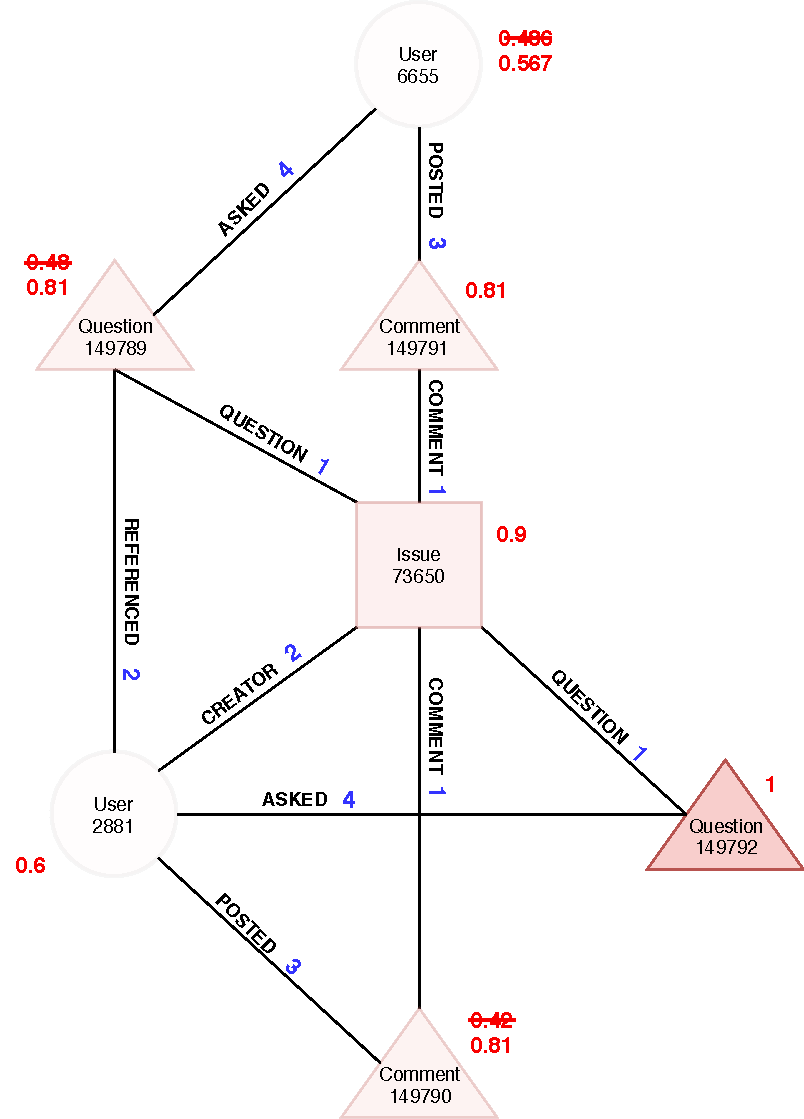
\includegraphics[width=0.85\linewidth]{RSTG-SA.pdf}
	\caption{Spreading Activation Applied to an RSTG (Without Frequency Bonus)}
	\label{fig:rstg-sa}
\end{figure}

The co-routine is divided into two branches by a conditional structure (Algorithm \ref{alg:spread}, Co-Routine, Line 2). If a node has no activation yet, the activation is simply spread to the new node. However, if a node already has activation, which activation is considered? Following the example of PFIS2~\cite{pfis2}, the higher activation value is spread. However, in order to incentivize frequency (in order to promote the Frequent Collaborator and Frequent Contributor patterns), if a node already has activation (i.e. the node has an existing relationship to the question), a percentage of that existing relationship is added to the new activation. Currently, this frequency reward is set to 1\% (Algorithm \ref{alg:spread}, Co-Routine, Line 1); otherwise, highly-central figures gained disproportionately high activations, and therefore activations did not suitably diminish throughout the graph. Another method for reinforcing frequent collaboration could be a subject for future work.

Figure \ref{fig:rstg-sa} provides an example of this variant of spreading activation being applied to the RSTG from Figure \ref{fig:rstg}. Each of the relationships is assigned its weight, and the activation of Question 149792 is set to 1. Then, User 2881 and Issue 73650 are visited and activation from the question is spread. Comment 149790 and Question 149789 had activation spread from both User 2881 and Issue 73650; the higher activation was retained. 

\section{Delineating Patches within Spreading Activation RSTGs}
With spreading activation encoding relatedness with the traceability forager's information need, patches can be created. Recall, from WUFIS and PFIS, that activation is a measure of information scent. By grouping together nodes with high activation, a patch with nodes related by the relationships described previously will be created. To do this, though, a threshold of ``high'' activation must be defined.

Earlier, creating patches by simply enclosing all nodes within four degrees of separation was proposed, because all answers in our dataset fell within four degrees. We now consider those answers' activations. Examining graphs of the classes discussed earlier, with spreading activation completed, reveals that a forager setting the cutoff at 0.72 would include 84\% of results. Setting the cutoff at 0.45 would include all results. Examining earlier classes revealed that many Frequent Contributors and their related information artifacts fall above 0.56; many Frequent Collaborators fall around 0.50.

\section{Results and Analysis}
\subsection{Quantitative Evidence}
Figure \ref{fig:resultsStats}, and samples taken from that figure in Table \ref{tab:resultsStats}, show us how big and how effective patches delineated by activation might be, similarly to Table \ref{tab:radiusStats}. In both, we provide descriptive statistics that tell us how large our patches would be if we only included nodes above a certain activation, as well as how many questions would contain their corresponding answers in that patch. While we don't see the inclusion of the answerer as necessary for an effective patch (as the patch should provide information other than a user who can answer questions), it does still provide a metric to show how relevant the patch might be.

The descriptive statistics in Figure \ref{fig:resultsStats} and Table \ref{tab:resultsStats} suggest that delineating patches by activation creates smaller patches than by degrees of separation (Table \ref{tab:radiusStats}). Statistically comparing 4 Degrees and Activation $\geq$ 0.45, we conclude that the two sets are non-identical (t = 10.901, p-value $<$ 0.01). A similar test for Activation $\geq$ 0.45 and $\geq$ 0.72 reaches the same conclusion (t = 9.6481 p-value $\geq$ 0.01). In other words, each cutoff has significantly smaller patches than the previous. 

\begin{figure}[ht]
	\centering
	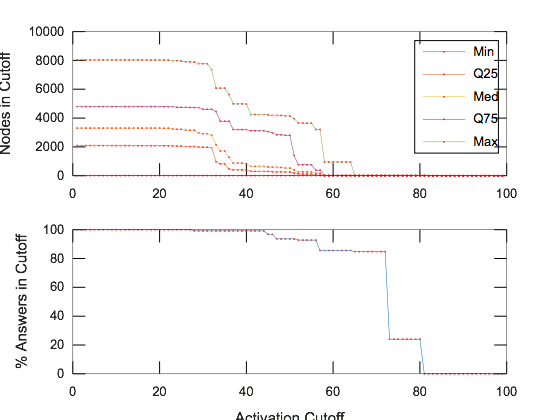
\includegraphics[width=\linewidth]{nodesincutoff.png}
	\caption{Patch Size With Cutoff}
	\label{fig:resultsStats}
\end{figure}

\begin{table}[ht]
	\caption{Patch Size With Cutoff (Samples from Figure \ref{fig:resultsStats})}
	\centering
	\begin{tabular}{ |c||c|c|c|c|c||c|  }
		\hline
		& Min & Q1 & Med & Q3 & Max & Answer \\
		\hline
		4 Degrees & 5 & 625  & 2288 & 3636 & 7542 & 100\% \\
		A $\geq$ 0.45 & 5 & 273 & 649 & 1860 & 4834 & 100\% \\
		A $\geq$ 0.50 & 5 & 190 & 406 & 1399 & 3961 & 93\% \\
		A $\geq$ 0.56 & 4 & 44  & 165 & 384  & 3207 & 85\% \\
		A $\geq$ 0.72 & 2 & 4 & 6 & 10 & 24 & 84\% \\
		\hline
	\end{tabular}
	\label{tab:resultsStats}
\end{table}


While patch sizes at cutoff Activation $\geq$ 0.45 are still too big for timely foraging, patch sizes at $\geq$ 0.72 are substantially more reasonable. That being said, $\geq$ 0.72 patches frequently do not include the answer node for three or four degree of separation relationships. However, within these patches, we believe that foragers would still find information relevant to their information need.

\subsection{Two Practical Examples}
Figure \ref{fig:rstg-sa} serves as a practical example of both the mechanism of the algorithm and a tradeoff to consider. Figure \ref{fig:rstg-sa} is a network with a cutoff set to $\geq$ 0.56\textemdash a cutoff chosen for its inclusion of many Frequent Contributors. Indeed, it was a Frequent Contributor that answered User 2881's question; User 6655 had commented twice on Issue 73650 already. While the question (``Does it work?'') was a pointed request, asking for a specific piece of information, the patch generated by the request yields not only the user who will answer the request, but also related traceability information\textemdash a history of work conducted towards that issue, leading to ``Does it work?''.

Figure \ref{fig:rstg-sa} also demonstrates a limitation of the algorithm in its current state. Other implementations of spreading activation begin from one or more nodes; we could have started the activation from the question \textit{and} the asking user. We chose to include only the question node, as to avoid superfluous information from the asking user's connections. In this case, though, had we included User 2881 as an initial node for activation, the algorithm would have assigned higher activations to the direct collaboration between User 6655 and User 2881 (User 2881--Question 149789--User 6655). This collaboration was key to the traceability history of Issue 73650.

\begin{figure}[ht]
	\centering
	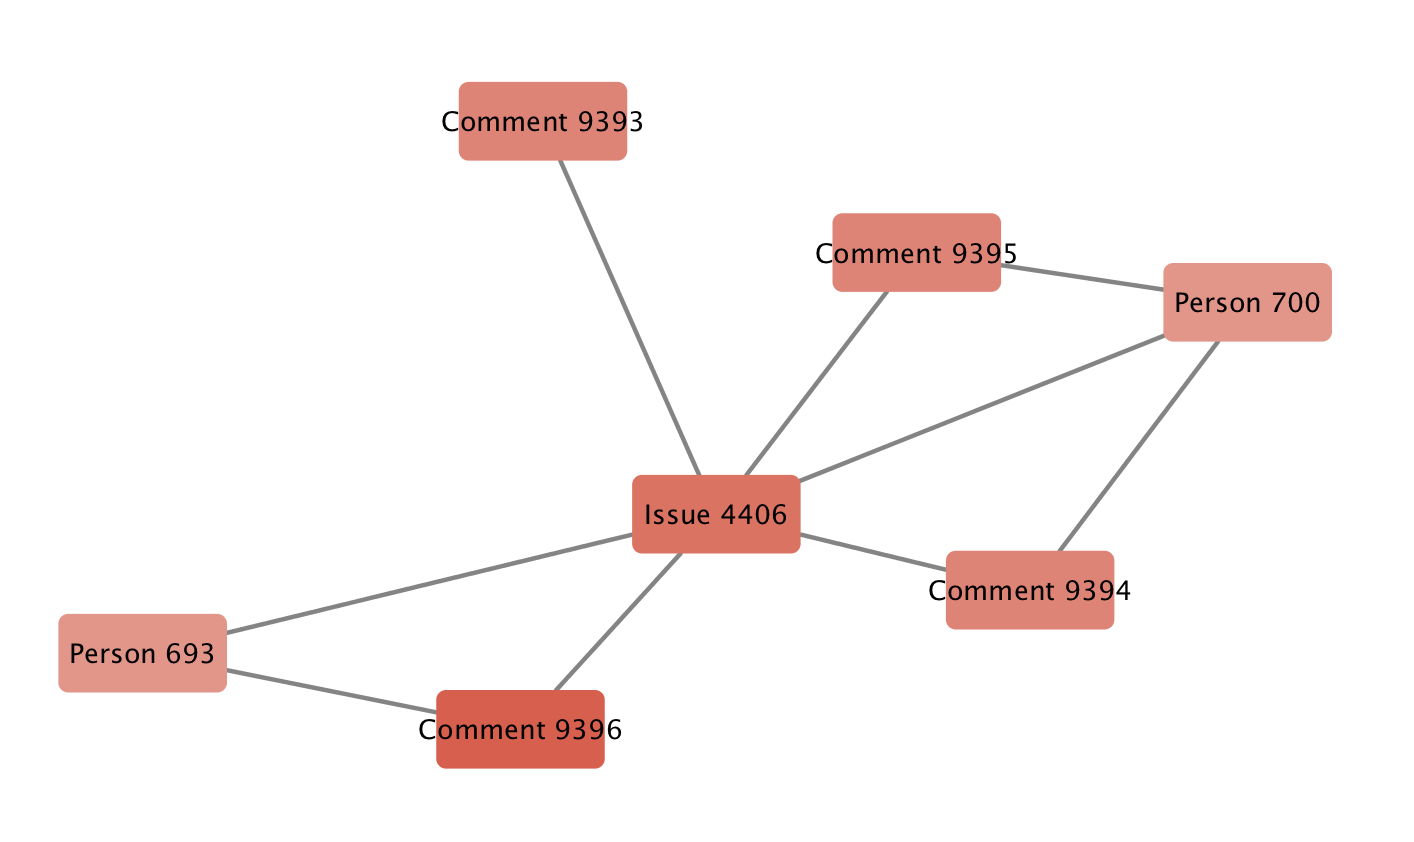
\includegraphics[width=\linewidth]{c9396weight_filter.png}
	\caption{Graph Generated from Comment 9396, A $\geq$ 0.72}
	\label{fig:cytoscapeFiltered}
\end{figure}

Another typical example, seen in Figure \ref{fig:cytoscapeFiltered}, demonstrates another interesting property of our algorithm. This figure was generated using the Cytoscape ~\cite{cytoscape} Network Analysis and Visualization tool, and was filtered to only show nodes with A $\geq$ 0.72. (This method is how we actually conducted our analyses described throughout this work.) The complete network, before filtering, can be seen in Appendix \ref{app:cytoscape}, Figure \ref{fig:c9396}. Intensity of color correlates to activation, with most intense color being A=1.

In this situation, the question posed was Comment 9396: ``Did this make it into PropertiesFactory?'', and Person 700, Gytis Trikleris, answered. While Trikleris did indeed make it into the patch, both he and the author were the lowest-activation nodes in this patch. In other words, thanks to the weighting assigned to commenters and askers, people do not have as high priority as information artifacts do. This could have interesting implications, not all necessarily positive--perhaps the current implementation of the algorithm might not be leveraging social connections as much as it should, and a better weighting scheme should be devised. We explore this further in the next section. 

The other interesting characteristic of this example is that the comments and people in the patch are all of the issue's commenters and contributors, and nothing from other issues. After examining neighboring nodes, we determined that this was the correct behavior\textemdash adding more nodes would have provided irrelevant information. Our algorithm, in many cases, provides only the neighbors to an issue, as those provide the highest degree of relevance to the question.